\chapter{Lvis - light transport visualisation library}\label{chap:vis}

We now present a C++ library that allows for selective visualisation of light paths generated by Metropolis Light Transport, or any other path or ray tracing algorithm. It allows the end user to control the volume of visualized data, provides control over the real-time scene visualisation in terms of camera positioning and lightning, supports interaction with mouse and keyboard, provides tools for path vertex position based filtering, mouse selection and visualisation-to-pathtracer feedback.

Since it was develop with MLT in mind, it also supports a set of features closely related to this method, namely the capacity to visualise a sequence of paths while highlighting mutated segments, and to provide the path tracer with a feedback in form of a user selected light path, which can than be used as a new basis for the next mutation. The aim of this library is to provide a tool for better understanding of existing mutation strategies and possibly also for development and debugging of a new ones.

\section{External libraries and requirements}

The library is written in C++, with the visualisation being handled by OpenGL, using the 3.0 standard - this being the highest OpenGL standard currently available to many Linux distributions and graphics cards (graphics card drivers in particular are the main issue here), or in other words, the highest version supported by the machine this library was developed on. As with most OpenGL applications, we rely on a set of additional libraries to provide us with the more standard functionality - GLEW to allow for hassle free use of the modern parts of OpenGL, GLM (OpenGL Mathematics) to provide us with the usual vector and matrix operations, SFML (Simple and Fast Multimedia Library) for context creation and input handling, DevIL (Developers Image Library) for texture loading and finally Assimp (Open Asset Import Library) for model loading. All of these are freeware, open source and cross-platform.

\section{Compilation and usage}

If you wish to compile and run a program using the Lvis library on your local workstation, you'll need all of the libraries mentioned in the previous section, along with their respective dependencies, installed. OpenGL 3.0 along with GLSL 1.3 support is also required. The enclosed Cmake file was tested on Ubuntu 14.04, but should work on any Linux distribution, and may require some minimal modifications for Windows. Your compiler must also support the C++11 standard.

In the path tracer (or other program you wish to use with Lvis), you first need to include \texttt{lvis/include/lvis.hpp} and create a new instance of Lvis object (with arguments to the constructor being path to scene file, and path to scene file textures). Then, whenever you wish to start the visualisation, you just need to call the run() method on your Lvis object. This creates the OpenGL rendering context in a new window, starts the visualisation and allows you to safely access all of the other public methods provided by Lvis. These will be explained in the subsequent sections (for correct usage, it is recommended to read at least the sections on threading and the section on light paths), with the example program provided in Chapter 3. 

\section{Implementation}

\subsection{Class Lvis}

The main class provides all the interfacing, between both the Lvis library and the path tracer, and user input and all other library classes. It holds all of the data structures (with pointers to the instantiations of other classes), and also contains methods for selection and path filtering. In this subsection we provide a categorised rundown of its functionality.

\subsubsection{Initialization}

While the constructor code only assigns paths to scene files to their respective variables, the initialization of OpenGL and member data occurs when \texttt{Lvis.run} is called. Context creation is handled by SFML, which has a rather streamlined approach towards it - the downside is having little control over some of the more advanced OpenGL settings, which we don't really need anyway. All of the shader files are loaded, compiled and linked at this point, and Assimp is used to parse every 3D model needed for the visualisation (more on this later). If there's an error at any stage of the initialization, program prints a warning and exits.  

\subsubsection{Threading, flags and public methods}

We take advantage of the C++11 standard and implement threading using the \texttt{std::thread}, \texttt{std::mutex} and \texttt{std::condition\_variable}. Multithreading is used so that the user can freely navigate and interact with the scene even while new light paths are generated. Data modifiable by both threads (expect for some of the flags, which we'll cover soon) are protected by a \texttt{std::unique\_lock} on a single mutex object, and condition variable is used to signal the path tracer thread after each draw cycle. The rest of the cycle being again protected by the mutex - since each of the functions may require an access to shared memory, and we're not too concerned about the time efficiency (and in fact, multiple lockings and unlockings may hinder it even further), it's much clearer to simply lock the whole block and allow path insertions only in-between renderings.

Communication between the two threads is provided by a set of public methods and also via \emph{flags} (boolean variables). The only threading-related method not associated with these flags at all is \texttt{Lvis.join}, whose use in the context of threads is fairly self-explanatory. The same can be said about the \texttt{flagRunning} and its related methods, while \texttt{flagSelected} and \texttt{flagSingle} simply signalize to the second thread that a new path was selected and should replace the current active one, or that we want to be pushing and visualising paths one after another, using the method \texttt{pushSinglePath} instead of the standard \texttt{pushPath}, respectively. The \texttt{flagPause} is a bit more interesting, and it's usage is left entirely on the end user. The idea, and proposed design, behind it is for it to be used in conjunction with \texttt{Lvis.wait} - which pauses the execution of a thread it was called from until signaled by \texttt{flagWaiting}. Since \texttt{flagWaiting} is private to prevent race conditions, we provide the user with \texttt{flagPause} to signal the path tracer thread whether it should call for \texttt{Lvis.wait}. An example usage (but not the \emph{only} right way to do so) of this flag is show in the demonstration program (\ref{lst:demo}), where it also provides different behaviour in conjunction with flagSingle. 

Apart from \texttt{Lvis.clearX} methods, which are again self-explanatory, we've yet to mention a couple of functions for further control over the visualisation and a set of methods limiting the data throughput. \texttt{Lvis.setupLight} allows us to position a single point light source, to allow for a closer match between lightning in visualisation and in the offline rendering. \texttt{Lvis.setupVirtualCamera} positions a camera model, facing a certain direction with the given up-vector, to match the camera used in the rendering. 

The last three of the public methods are \texttt{Lvis.setLimit}, \texttt{Lvis.setDrawLimit} and \texttt{Lvis.setThreshold}. As their name imply, each of these modifies a certain parameter - or a certain limit - of Lvis class. \texttt{limit} is the maximum number of paths that can be stored inside \texttt{std::vector inputPaths} (those are the paths waiting to be filtered and drawn), \texttt{drawLimit} is the maximum number of paths drawn in the scene at each point in time and finally, \texttt{threshold} is the minimal size of \texttt{inpuPaths} before it can be filtered and subsequently drawn.

\subsubsection{Input, selection \& colour picking}

All of the keyboard and mouse inputs are handled by SFML. This is done in two ways,the first one is through the \texttt{sf::Event} class, which polls the window class for all mouse, keyboard and window events (including window resizing or closing). The advantage of this approach is that only inputs that happen inside the window (or while the window is focused) are registered, but on the other hand, the keyboard events are triggered only when the key is pressed or released. To implement continuous camera movement (via keyboard), we use the \texttt{sf::Keyboard} class, which allows for real-time feedback, but we need to check for window focus on our own.

Left mouse button clicks triggers the selection mechanics - we need to differentiate between clicking one of the axis of the active sphere selector, other selector, light path and any other place on the scene. This was implemented through the use of off-screen rendering and colour picking. For axes it's pretty straightforward, since we're reading \texttt{RGB} values and each axis occupies only a single channel. Each of the spheres and paths have a unique id, which is assigned using the \texttt{counter} variable and \texttt{Lvis.counterUp} method\footnote{Note that this means there is no overlap in the ids of spheres and paths, and since we're clearing the colour buffer each time we're selecting a new object, we could have used different counters for different shapes, allowing us to draw slightly more paths at once. But since the number of used selectors will always be much smaller than the number of drawn light paths (unless we choose to draw a small number of paths, in which case this is of no concern at all), we use a single counter for convenience.}. This id is then ``hashed''  into an \texttt{RGB} colour (this idea was taken from \cite{ColorPicking}), which is then used to draw the object during the picking stage. Spheres are, of course, drawn as solid objects instead of wireframes during this step. The picked colour is then used as a key value for the relevant map structure.

\begin{listing}
\begin{minted}[mathescape,
               numbersep=5pt,
               frame=lines,
               framesep=2mm]{c++}
r = index&0xFF;
g = (index>>8)&0xFF;
b = (index>>16)&0xFF;
\end{minted}
\caption{Encoding index into RGB color for picking.}
\label{lst:hash}
\end{listing}

\subsubsection{Selector positioning and movement}

Every new sphere selector is created at the position of virtual camera (defaults to scene origin) - this seems like a good place to start since it's also the place where all of the paths generated by bidirectional tracers will end. While the actual translation, in terms of modifying its Model matrix, is done inside the \texttt{SphereSelect} class, the values passed to it are determined in the \texttt{Lvis} class, therefore we now present their calculation to you.

When the selector is active (i.e. it has been clicked on), it displays coloured arrows along each of the three axes of the object coordinates (we've actually nicknamed these arrows as ``axes'' in the source code and already referenced them like that in this paper, so might as well carry on with it). The green one is always oriented towards the positive y-axis, while the other two switch from positive to negative depending on the camera position (to allow for easier manipulation).

When dragging the sphere along one of the axes, the direction is decided this way - first, we use the same Model - View - Projection (MVP) matrix that we've used to display the sphere to get the window coordinates of our vector. This transformation is applied to a vector of homogeneous coordinates, where the \emph{w} (the fourth value) is set to \emph{zero}. This way, all of the translations contained in the MVP matrix are omitted, and the vector we get from this transformation will have it's origin in the center of the screen, pointing towards one of the four quadrants. Based on this information, we either translate along the arrow, when the mouse cursor is moving towards that quadrant, or in the opposite direction if it's moving away from it. This is done separately for the x and y directions, so for example, if the transformed vector lies in the first quadrant, dragging it both upwards and to the right side moves the sphere along the arrow. The same applies for scaling. 

\subsubsection{Drawing}

All of the actual drawing (i.e. the binding of VBOs and calling \texttt{glDrawElements} or \texttt{glDrawArrays}) is performed in other classes, \texttt{Lvis.draw} simply iterates through all of their instances and calls the appropriate methods. It is also responsible for setting the uniforms for camera position (that is, the position of actual OpenGL camera, for use in the Phong shader) and light position, and choosing the appropriate shader for drawing the scene.

\subsection{Camera}

In modern OpenGL, we're no longer forced to use the built in ModelView and Projection matrices. Instead, developers are encouraged to implement these matrices by themselves, with GLM becoming the standard library for creation and manipulation of both the matrices and the vectors they are transforming. The primary function of \texttt{Camera} class is to hold the View and Projection matrices, and provide functions for their manipulation. Because of our grouping of these matrices in a single class, we commonly retrieve a single \emph{ViewProjection} matrix (using the \texttt{Camera.getVP} method), and then use the positional attributes of the objects in scene to construct a model matrix (if needed).

\begin{figure}[h]
    \centering
    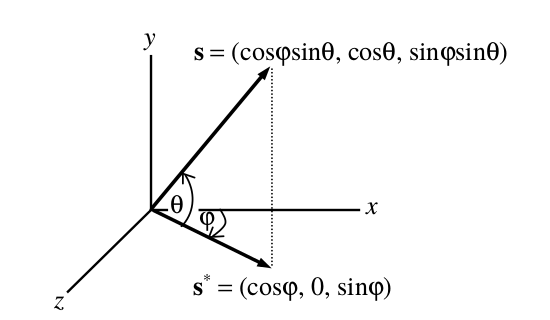
\includegraphics[width=0.5\textwidth]{spher.png}
    \caption{Spherical coordinates, image courtesy of doc. RNDr. Miloš Božek, PhD.}
    \label{fig:spher}
\end{figure}

Camera can operate in two different modes, the default one is always facing the center of the scene, while the \emph{free mode}, as the name suggests, allows for free movement around the scene and rotation around the camera origin. Rotation is represented in spherical coordinates (fig. \ref{fig:spher}, the difference being that we use \texttt{xi} and \texttt{fi} in place of $\theta$ and $\varphi$, respectively ). Since in \texttt{Lvis} class, this rotation is performed by dragging the mouse, and only the most recent position values are sent, we need to remember the angles set before the rotation began, which is done through the use of \texttt{Camera.memorizeSpherical}. 

In the default mode, the unit vector calculated from these angles is multiplied by the desired distance from the center and then used to position the camera, while in the free mode, the position is controlled via the keyboard input, and the unit vectors are used to set the viewing direction. We use \texttt{glm::lookAt} method to compute the View matrix in both approaches, along with \texttt{glm::perspective} to construct the desired Projection matrix.   
 
\subsection{Shaders}

Before introducing the drawing procedures, let us present a quick rundown of the shader programs used by the library. \texttt{lineProgram} is the simplest one, only performing the standard Model-View-Projection transformation in vertex shader, and colouring each fragment with the colour passed as a uniform (same for each fragment in the whole mesh). As the name indicates, it's used primarily for drawing polylines (light paths), but also for drawing sphere selectors and axes, since no further functionality is required there. For scene (and virtual camera) drawing, one of the three shader programs is used - \texttt{basicProgram}, \texttt{noTextProgram} or \texttt{textOnlyProgram}. They all share common vertex shader and data structure, therefore differentiating only in fragment shader code. The basic shader combines texture sampling with Phong model ambient,diffuse and specular contributions, \texttt{noTextProgram} omits the texture and similarly, \texttt{textOnlyProgram} forgoes the lightning calculations. The user can switch between these three at runtime.

\subsubsection{Phong illumination model}

Implementation of the fragment shader was taken from an online tutorial \cite{OGLAssimp} - since the computation is given by a single, standardized formula, no changes were needed. This formula (in our implementation, which uses only a single light source, and we also omits most of the material constants, using the same formula for all objects and materials) goes as follows
\begin{align*}
I_p = i_a+(L.N)i_d+(R.C)^{\alpha}i_s
\end{align*} 
where $i_a$, $i_d$ and $i_s$ are vectors containing the ambient, diffuse and specular components of lightning (in our case, they are set to \texttt{(0.05,0.05,0.05)}, \texttt{(0.7,0.7,0.7)} and \texttt{(1.0,1.0,1.0)} respectively), $\alpha$ is the shininess constant (again, set tu \texttt{4.0} for all the materials) and $I_p$ is in our case the resulting brightness of a fragment (since our $i_a$, $i_d$ and $i_s$ are all represented as intensities of white light). Rest of the equation consists of normalized vectors and their dot products, where $N$ is the surface normal, $L$ is the direction towards the light source, $R$ is the direction that a perfectly reflected ray of light would take and $C$ is the direction towards the camera, all of these pointing from the currently processed surface point. In the \texttt{basicProgram}, this value is then multiplied by a value sampled from the appropriate texture at given UV coordinates. In \texttt{noTextProgram}, the whole calculation is omitted.

\subsection{Assimp, sceneLoader and meshes}

Let us first provide you with a brief note on Assimps internal data format. After loading the model file with desired flags - in our case, we're flagging to triangulate (since our OpenGL standard supports only triangulated meshes), calculate tangent space and calculate normals (both for the use in Phong shading model) - we are left with a \texttt{aiScene} object. This object contains a pointer to \texttt{aiNode} tree structure, with each node containing a certain set of data, out of which we're only concerned for an array of meshes. Therefore, we traverse the tree structure and parse every mesh into our mesh class format, processing all the vertices, indices, textures with its coordinates, normals and tangents (in \texttt{sceneLoader}), and afterwards creating VBOs (for vertices and indices) and binding the data to them (in mesh class). Both of these classes were again taken from an online tutorial \cite{OGLAssimp}, and only slightly modified to our needs - i.e. the original file used SDL for texture loading - instead, we opted to use DevIL as a more lightweight alternative - and we also added an option in the \texttt{sceneLoader.draw} and \texttt{mesh.draw} functions to draw wireframe model instead of a solid one (for use in sphere selectors).

When drawing the scene, first the shader program is chosen and uniforms containing light and camera positions are set. All of this happens in the \texttt{Lvis} class, which then calls the draw function of \texttt{sceneLoader}, along with the shader program id and ProjectionView matrix gathered from the \texttt{camera} class. The \texttt{sceneLoader} class simply calls the \texttt{sceneLoader.draw} function of all of the meshes associated with it, delegating the data passed to them from the previous class. And finally, actual binding of vertex data and drawing (call to either \texttt{glDrawElements} or \texttt{glDrawArrays}) happens in the \texttt{mesh} class. We are using \texttt{drawArrays} insted of \texttt{glDrawElements} when drawing wireframe to conserve a bit of data transfer between CPU and graphics card - since we're already doing a lot more of it by replacing a single call by one for every triangle. The drawing of virtual camera, spheres and their axes looks almost exactly the same, except that we add another step inside these classes to allow for further modifications to MVP matrix and shader uniforms.

\subsection{Sphere selectors}

Already mentioned a couple of times in this paper, \texttt{sphereSelector} class allows us to filter through the drawn, and about-to-be-drawn light paths. The filtering is done based on the distance from the center of the selector, therefore they are visually represented by a sphere (iconosphere wireframe in particular, since again, we're only allowed for triangulated surfaces in the newer OpenGL, and we want the model to be wireframe for practical purposes). The spheres are all created with the radius of \texttt{1.0}, which is then (together with the actual area of effect) controlled by the variable \texttt{scale}. 

At this point, we should explain how the scaling and translation works from inside of the \texttt{SphereSelect} class (the way that the values for these operations are passed was already discussed in the \texttt{Lvis} class subsection). We use a slightly different system than in \texttt{Camera} class, but in the end, both of them are practicaly the same thing, just taken from a different angle. While with the \texttt{Camera} we saved the \texttt{oldXi} and \texttt{oldFi} at the start of the operation, here we have \texttt{glm::vec3 tempTrans} for translation and \texttt{tempScale} for scaling, which are rewritten by every call of \texttt{SphereSelect.translate} and \texttt{SphereSelect.scaling} respectively, and are only written into their ``permanent''  counterparts when \texttt{SphereSelect.finishTranslate} and \texttt{SphereSelect.finishScaling} are called. The downside of this being that we need to use both the temporal and the permanent variable to the transformation matrices, to provide the user with feedback.

All of the actual filtering is done via the function \texttt{pointInside}, which calculates the distance between the center of the selector and the point passed as a parameter (usually a position of a \texttt{PathVertex}), and returns a boolean value based on the \texttt{scale} and the result of this calculation. The library provides four basic kinds of selectors, three of them - the green (start), red (end) and yellow (any) selector work as if all of the selectors of the same kind made a logical statement containing only binary \texttt{OR} directives - therefore, if a single path vertex lies in any one of the selectors (still talking about one kind only), the whole statement is resolved as \texttt{TRUE} and the path is drawn. Similarly, we have one more kind of selector, the white one, which works as if all of them were in a logical statement containing only binary \texttt{AND} - so that path is only drawn if at least one vertex lies in every single white selector in the scene. The implementation of this algorithm can be found in the \texttt{Lvis} class (as a part of the \texttt{Lvis.filterPath} method).

Since spheres are to be selectable by a mouse click, this class also contains methods for transforming index number into \texttt{RGB} colour and vice-versa, for the use in picking algorithms, again located in the \texttt{Lvis} class.  

\subsection{Light paths}

Each light path is represented by a single instance of its class, which in turn consists primarily of the vector of pointers to \texttt{pathVertex} instances, which store a single \texttt{glm::vec3} object with vertex position. There are two reasons for having vertices as separate classes - the primary one during the development was the ability to swiftly create a randomized light path for debugging purposes, and the reason they've stayed in the later stages of the development cycle being the delegation of \texttt{PathVertex.getInfo} and the overall tidiness of the code. 

The light path is set up by appending new vertices from the start towards the end (note that sphere selector differentiates between the two boundaries). When we are ready to visualize the path, we must first call the \texttt{LightPath.finalize} method, to generate and bind a new VBO for the path. If we're doing this repeatedly, the previous VBO buffers are correctly deleted. If we try to add a new vertex after finalizing the path, it will be again marked as incomplete and won't allow us to visualize it before calling \texttt{LightPath.finalize} on it again. This method also creates an info log about the path, that we can then retrieve as a string.

Since we're adhering to the OpenGL 3.0 standards, where geometry shaders were still not the part of the core specification, and \texttt{glLineWidth} was not yet considered deprecated, we're being lazy and using this function to give our paths desired width, which can be set by the end user. Just like \texttt{SphereSelect}, \texttt{LightPath} contains methods for determining pick colour.

\subsection{Virtual Camera}

The final touch to the visualisation is in adding the model of a camera to a place where the camera of the offline renderer is positioned in the scene. This is set via the method \texttt{VirtualCamera.lookAt}, which takes the same parameters as Mitsubas, and probably also other renderers, lookat xml directive - therefore, if we're using our library in conjunction with such library, it is straightforward to correctly setup our virtual camera model.

\texttt{VirtualCamera.lookAt} uses another method to help with the correct positioning - \texttt{VirtualCamera.faceVector} - which takes two vectors as an argument, and returns the rotation matrix, that transforms the orientation of the first one to be the same as that of the second one. This is done by normalizing the vectors, after which their dot product will be equal to the cosine value of the angle between them, and then computing the cross product to get the axis perpendicular to both of them, around which we, finally, perform the rotation. 

To get the model, which was originally facing towards the positive infinity on the z-axis, with up vector lying on the positive part of the y-axis, to look at the desired position, we first need to obtain the direction we want it to be facing - by subtracting the \texttt{from} position vector from the \texttt{to} vector. We can ten perform the rotation (provided by the \texttt{faceVector} method) from the default facing to the new one. We also perform the same rotation on the default up vector - to find out what will the up vector look like after this transformation. From that we get the new \texttt{tmpUp} vector, and we need to again find a rotation matrix that transforms it to our desired up vector - which we'll do again by the same method as before. As a last step, we translate the camera model to the desired position, and apply all of these operations to the ViewProjection matrix of the OpenGL camera. Also, before any of these transformations , the whole model is scaled down and translated so that it's lens are at the initial model coordinates origin - this is the place were all of the light paths will end.